\section{Introducción}

\subsection{¿Qué es la visión artificial?}

Los seres humanos somos capaces de percibir con facilidad el entorno tridimensional que nos rodea \cite{tfg}. El funcionamiento exacto de nuestra visión (y, asimismo, de nuestro cerebro)  ha sido fruto de investigación exhaustiva por parte de la comunidad científica \cite{book:szeliski}. Psicología, oftalmología, neurociencia e incluso ingeniería son algunas de las ramas que investigan sobre nuestra visión sin, de momento, llegar a una respuesta concluyente.

La idea de visión artificial surge a finales de la década de los 60. Desde entonces, se han desarrollado técnicas matemáticas para todo tipo de aplicaciones. En la actualidad, entre las aplicaciones más avanzadas se encuentra el reconocimiento, detección y clasificación de objetos o elaboración de descripciones verbales utilizando imágenes.

A pesar de estos avances, la tarea de hacer que un ordenador llegue al nivel perceptivo de un niño sigue siendo un objetivo más bien lejano. La dificultad de la visión por computador es, en ocasiones, subestimada. Se suele tender a pensar que la parte más complicada de un sistema de inteligencia artificial son las partes cognitivas y no las relativas a la percepción, aunque tienen dificultades similares entre sí.

La dificultad de la visión artificial radica, de hecho, en nuestro desconocimiento del funcionamiento de la nuestra. Esto lo convierte en un problema más bien de ingeniería inversa: utilizando una cantidad de información insuficiente, como una imagen, se trata de llegar a las incógnitas que permiten encontrar la solución completa. En otras palabras, el objetivo es reconstruir no sólo las propiedades de los objetos (forma, iluminación, color...), sino también el reconocimiento (clasificación) de los objetos, la separación de unos objetos de otros (segmentación), etc.

Ahora bien, no todo son malas noticias: la visión por computador tiene numerosos casos de uso hoy en día. Entre sus aplicaciones encontramos cosas como (\citeauthor*{book:szeliski}):
\begin{itemize}
  \item \textbf{Reconocimiento de caracteres óptico.} Se ha llegado a reconocer caracteres numéricos con una tasa de error del 0.16\% \cite{byerly2020branching}.
  \item \textbf{Inspección mecanizada.} Inspección de partes de automóviles o aeronaves a fin de, por ejemplo, encontrar defectos en el metal o generación de modelos 3D a partir de escaneos (Figura \ref{fig:apps1a}).
  \item \textbf{Construcción de modelos 3D.} Construcción automatizada de modelos 3D a partir de fotografías aéreas como las que usa Google
        (Figura \ref{fig:apps1b}).
  \item \textbf{Seguridad en automóviles.} Reconocimiento de obstáculos tales como peatones u otros coches, en condiciones en las que el radar o el lídar no funcionan bien, en tecnologías como \href{https://www.mobileye.com/}{Mobileye}.
  \item \textbf{Reconocimiento de huellas dactilares y biométricas.} Usado ampliamente hoy en día en teléfonos móviles.
  \item \textbf{Reconocimiento y localización de objetos, categorías y acciones.} Usando deep learning, se ha conseguido un cierto grado de precisión a la hora de reconocer objetos dispersos en una escena.
\end{itemize}

\begin{figure}
  \begin{subfigure}{.5\textwidth}
    \centering
    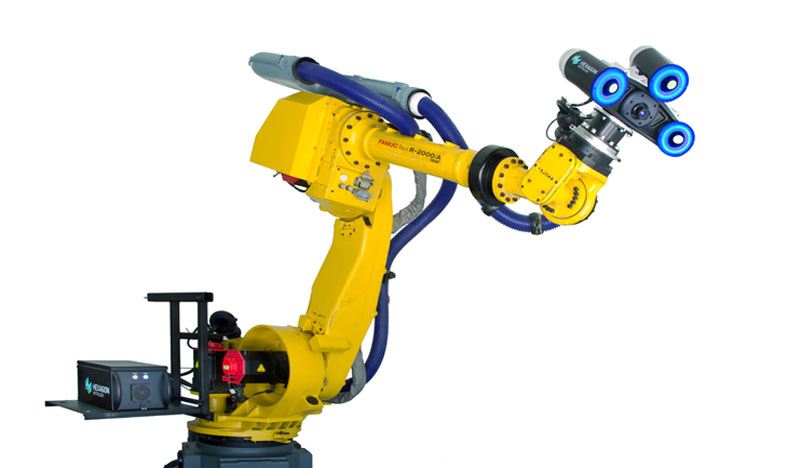
\includegraphics[width=.9\linewidth]{images/camera.jpg}
    \caption { }
    \label{fig:apps1a}
  \end{subfigure}%
  \begin{subfigure}{.5\textwidth}
    \centering
    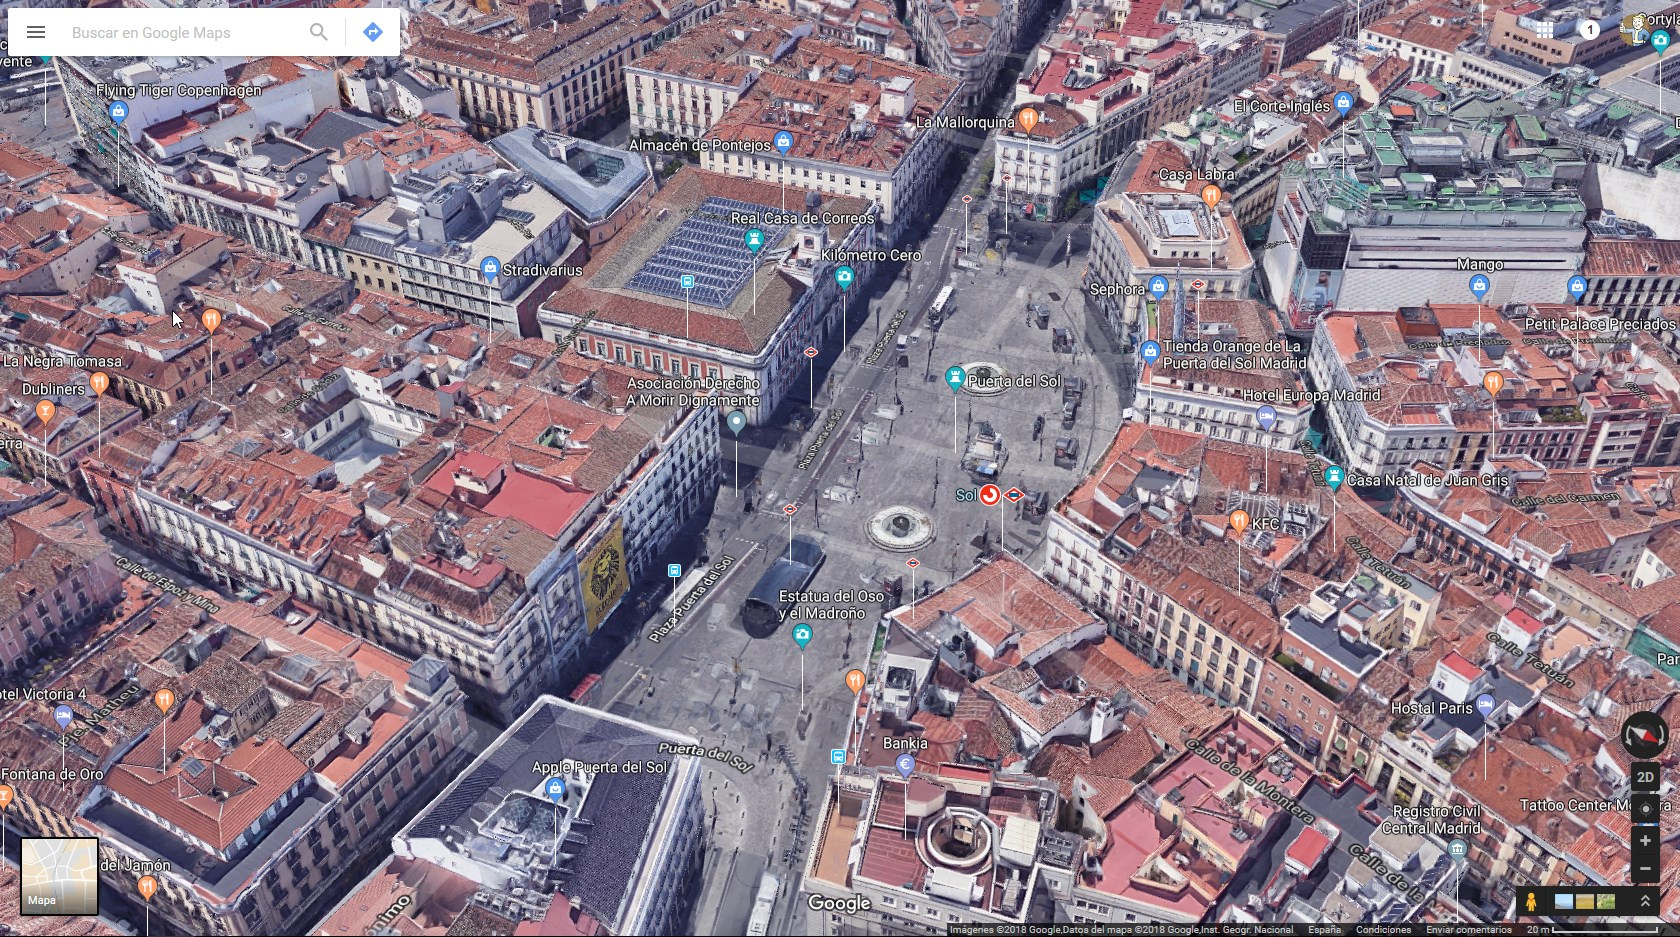
\includegraphics[width=.9\linewidth]{images/maps.jpg}
    \caption { }
    \label{fig:apps1b}
  \end{subfigure}
  \caption{Algunas aplicaciones de la visión artificial: (a) sistema de escaneado de objetos por luz azul \href{https://www.hexagonmi.com/es-ES/products/white-light-scanner-systems/blaze-600a}{BLAZE 600A}. (b) reconstrucción 3D en Google Maps de la Puerta del Sol \cite{tfg}. }
  \label{fig:applications}
\end{figure}

\subsection{Breve historia de la visión artificial}

\begin{figure}[H]
  \centering
  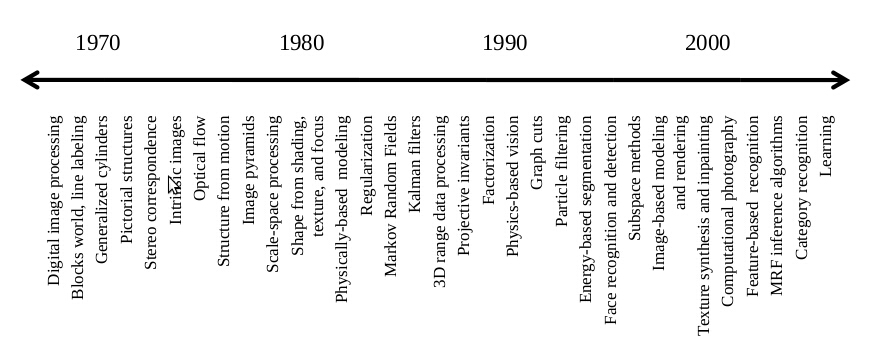
\includegraphics[width=0.8\textwidth]{images/timeline}
  \caption{Timeline de las aportaciones más importantes a la visión artificial \cite{tfg, book:szeliski}.}
\end{figure}

La primera vez que surge la idea de visión por computador es en 1966, cuando Marvin Minsky le asignó a su alumno en el MIT Gerald Jay Sussman un proyecto de verano en el que le encargó enlazar una cámara a un ordenador, haciendo que el ordenador describiera los objetos que se le presentaban a la cámara.

En la siguiente década, \textbf{en los 70}, la investigación en visión artificial comienza a tomar forma. En esta época, los pioneros en el campo de la IA y la robótica creían que resolver el problema de la entrada visual sería un trabajo fácil hacia la resolución de problemas de mayor envergadura. 

Lo que distinguió la visión por computador del campo del procesado de imágenes digitales fue la intención de reconstruir la estructura tridimensional del mundo a partir de las imágenes. Los primeros intentos en este sentido estaban relacionados con la extracción de ejes y posterior inferencia de la estructura 3D del objeto.

En \textbf{los 80} la investigación se centró en desarrollar técnicas matemáticas más sofisticadas para el análisis. Comienzan a usarse técnicas como las pirámides de imágenes. Se continuó con la investigación sobre la detección de bordes y contornos. Se empiezan a adoptar técnicas de detección de formas a partir de características de la imagen como las sombras, la textura o el enfoque. Estas técnicas fueron generalizadas utilizando el mismo modelo matemático al plantearlas como problemas de optimización. Aparecen también las primeras redes neuronales aplicadas a visión artificial.

En la \textbf{década de 1990} continuó la investigación en todo lo anteriormente mencionado. Hubo un esfuerzo por solucionar el problema de la estructura a partir del movimiento (\textit{structure from motion}). El trabajo de la década anterior que consistía en usar medidas color e intensidad en combinación con modelos físicos acabó por convertirse en su propio campo de investigación, llamado visión artificial basada en la física. Los algoritmos de \textit{tracking} mejoraron, surgen técnicas como \textit{mean shift}. Normalmente se aplicaron al seguimiento de caras o de cuerpos completos.

La segmentación semántica de imágenes fue un tema de investigación activo. Comienzan a aparecer técnicas de aprendizaje basadas en estadística, de las que surgen los primeros algoritmos de reconocimiento facial.

El avance más notable en esta década fue la interacción con la computación gráfica. La idea de crear animaciones desde imágenes tomó forma mediante técnicas de \textit{morphing}. A la vez, empezaron a introducirse técnicas capaces de obtener un modelo 3D a partir de colecciones de imágenes.

Durante la \textbf{década de los 2000} continuó la interacción entre el campo de la visión y el de los gráficos. En esta década proliferaron técnicas basadas en el uso de \textit{features} para el reconocimiento de objetos. Estas técnicas también dominan otras tareas del reconocimiento como el reconocimiento de la escena o de localización.

A finales de la década comienzan a aplicarse las técnicas de \textit{machine learning} a problemas de visión artificial, como es el uso de redes neuronales convolucionales. El crecimiento de esta técnica, de gran importancia en la actualidad, coincide con la gran disponibilidad en Internet de enormes cantidades de datos etiquetados, así como la multiplicación exponencial de la capacidad de cómputo, que hizo más rápido el diseño y testeo de modelos de redes neuronales.

Al igual que en el campo del \textit{machine learning}, las redes neuronales han cobrado una importancia vital, y se ha logrado avances verdaderamente grandes haciendo uso de ellas. Un ejemplo del estado actual del campo es el trabajo de \citet{art:2017arXiv170306870H} que muestra el avance en segmentación de imagen que se ha logrado usando ANNs (\textit{Artificial Neural Networks}).

También hay avances en la conducción autónoma usando visión por computador, de hecho NVIDIA tiene actualmente en funcionamiento una plataforma para coches autónomos llamada NVIDIA DRIVE. Dicha plataforma, nuevamente, hace uso de técnicas de deep learning para detectar obstáculos, señales, etc.

\subsection{El \textit{deep learning} y su aportación a la visión artificial}
\subsubsection*{Orígenes de las ANN}

El término \textit{deep learning} se refiere al conjunto de técnicas basadas en redes neuronales que permiten a un ordenador aprender a resolver una tarea concreta mediante el aprendizaje automático. En esencia, es una forma de \textit{machine learning}. Dichas redes neuronales permiten crear modelos capaces de extraer \textit{features} abstractas de alto nivel, como pueden ser caras, voces o coches, a partir de conceptos más sencillos como el color, los contornos o las esquinas (\citet{book:Goodfellow-et-al-2016}).

El concepto de red neuronal no es en absoluto novedoso, ya en 1943 el neurólogo Warren McCulloch y el matemático Walter Pitts las propusieron en un artículo \cite{art:mcculloch1943logical} en el que se presentaba un modelo computacional de cómo las neuronas biológicas funcionaban en conjunto para realizar cálculos complejos utilizando lógica proposicional.

Los éxitos iniciales de las ANN llevaron a la creencia de que una IA plena era inminente. Sin embargo, en los años 60 se vio que esto no iba a ocurrir pronto, así que las ANN quedaron en espera hasta los años 80, cuando se desarrollaron nuevas arquitecturas y técnicas de entrenamiento que llevaron a revivir el interés. En los años 90 se propusieron técnicas de machine learning como las máquinas de soporte vectorial (SVM), las cuales ofrecían mejores resultados (y más comprensibles) que las redes neuronales, así que volvieron a caer en el olvido.

En las dos últimas décadas ha habido una nueva oleada de interés por las redes neuronales, que podría ser la definitiva debido a varios factores. Primero, la gran cantidad de datos disponible para el entrenamiento de este tipo de modelos disponible en abierto en Internet, junto con el aumento de la capacidad de procesamiento, en gran parte porque la industria del videojuego ha estimulado la producción de cada vez mejores GPUs, que aceleran mucho el entrenamiento de este tipo de modelos. Gracias a estos factores, las redes neuronales han entrado en un circulo virtuoso donde los éxitos generan más interés, que se traduce en mayor financiación, que a su vez llevan a nuevos progresos.

\begin{figure}[H]
  \centering
  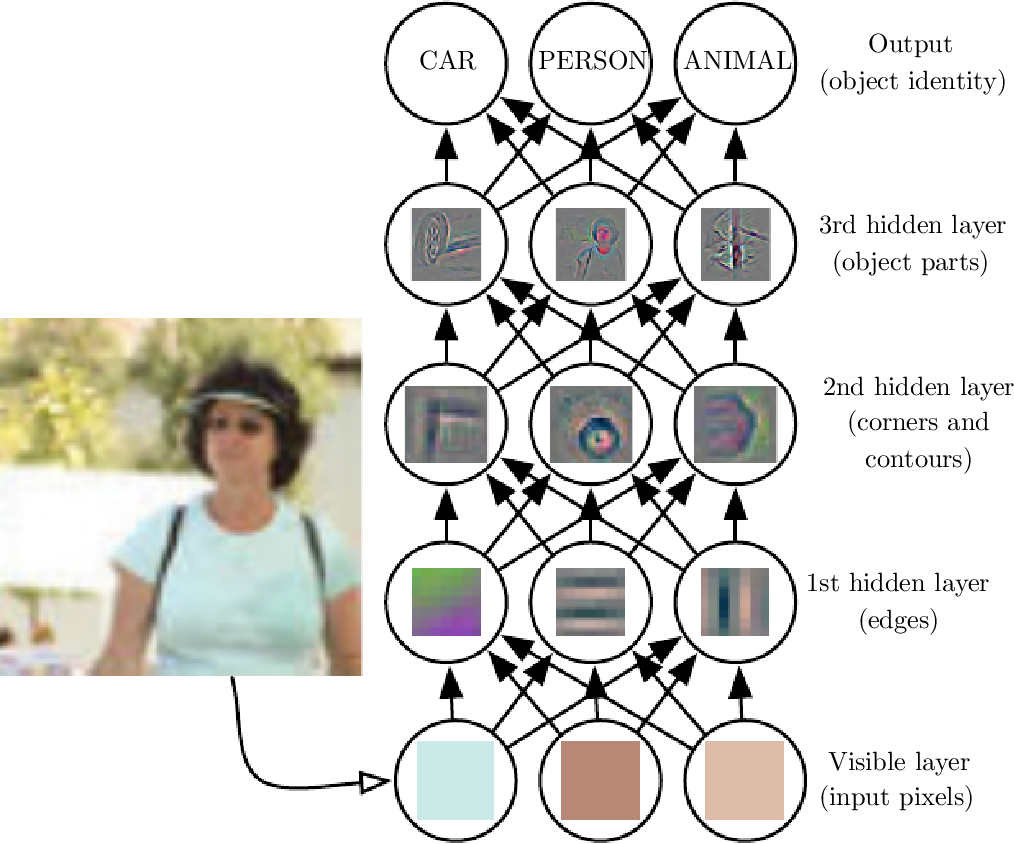
\includegraphics[width=0.6\textwidth]{images/mlp}
  \caption{Esquema de funcionamiento de un MLP \cite{book:Goodfellow-et-al-2016}.}
  \label{fig:mlp}
\end{figure}

El ejemplo más típico de un modelo \textit{deep learning} es el perceptrón multicapa (MLP, figura \ref{fig:mlp}), el cual consiste en una serie de una serie de nodos conectados entre sí a través de una o más capas, denominados neuronas. Cada una de dichas neuronas es, en realidad, una función matemática que, en la última capa, produce una salida. Esta salida se utiliza en un proceso denominado retropropagación (\textit{backpropagation}) del error cuyo objetivo es el de reajustar los pesos de cada uno de los perceptrones o neuronas que se hallan en el modelo, de forma que se reduzca el error en sucesivas iteraciones. Este algoritmo se propuso en 1987 \cite{art:backpropagation} y sigue siendo utilizado hoy en día.

El entrenamiento de una red neuronal utilizando retropropagación hace que en cada iteración (época) del entrenamiento se hagan dos pasadas a través de la red neuronal, una hacia delante donde se hacen las predicciones y otra hacia atrás donde se van ajustando los pesos que han afectado a dichas decisiones para subsanar errores. Este proceso se va repitiendo hasta que se converge en una solución.


Este proceso visto en detalle tiene los siguientes pasos \cite{book:homl}:
\begin{enumerate}
  \item Se procesa el dataset completo en cada época, dividiéndola en lotes (\textit{batch}).
  \item Cada lote pasa por la capa de entrada de la arquitectura, que la envía directamente a la primera capa oculta. El algoritmo computa la salida de todas las neuronas de la capa, que se obtiene mediante la ecuación:
  \[
    h_{W,b}(X) = \Phi(XW+b)
  \]

  Donde X es la matriz de datos de entrada; W es la matriz de pesos, que está formada por tantas filas como neurona de entrada y tantas columnas como neuronas en la capa; b es el vector de sesgo, con un elemento por neurona y $\Phi$ es la función de activación. La salida de la capa se utiliza como datos de entrada para la siguiente capa, repitiendo el proceso descrito hasta la capa de salida.
  
  \item Una vez obtenida la salida de la última capa para cada uno de los elementos del lote, se mide el error del modelo mediante una función llamada de pérdida (\textit{loss}) y se computa cuánto contribuye cada conexión de salida al error aplicando la regla de la cadena. A continuación se progresa hacia atrás aplicando la misma regla.
  \item Utilizando los gradientes de la función de error que se han computado en el paso anterior para cada capa, el algoritmo actualiza los pesos de cada neurona utilizando un algoritmo de descenso de gradiente.
\end{enumerate}



\subsubsection*{Uso de las redes neuronales convolucionales para visión computacional}

\begin{figure}[H]
  \centering
  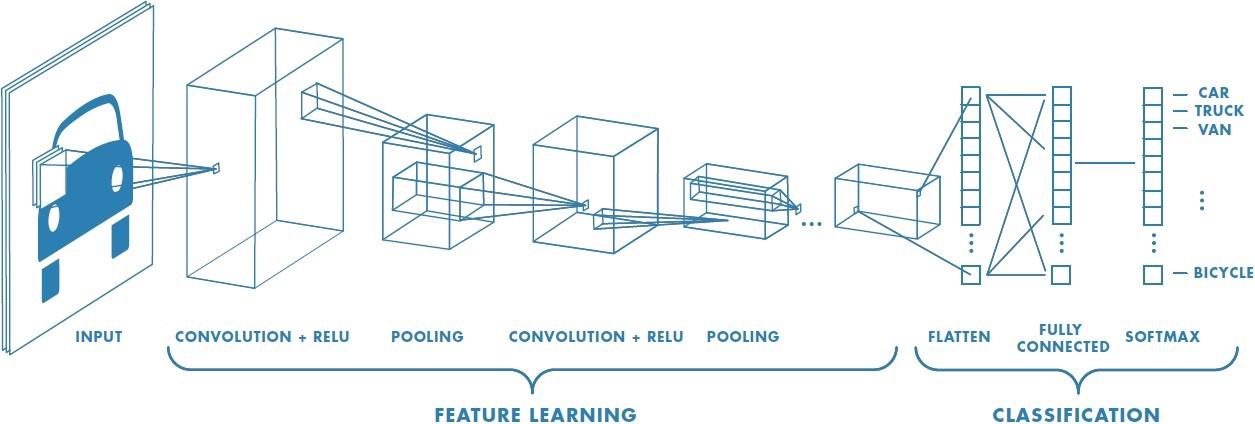
\includegraphics[width=0.6\textwidth]{images/cnn}
  \caption{Esquema de funcionamiento de una CNN \cite{mathWorksCnn}.}
  \label{fig:cnn}
\end{figure}

En 1958 \cite{art:cat58} y 1959 \cite{art:cat59}, David H. Hubel y Torsten Wiesel llevaron a cabo una serie de experimentos sobre el córtex visual de los gatos. En ellos se halló la cantidad de neuronas que se encuentran en dicho córtex y cómo este funcionaba: las neuronas del córtex tienen un pequeño campo receptivo sobre todo el campo visual y la combinación de todos los campos receptivos es el campo visual total. Además, algunas neuronas reaccionaban a imágenes de líneas horizontales y otras a líneas verticales, mientras que otras neuronas tenían un campo receptivo mayor, de forma que combinaban estos patrones de bajo nivel en otros más complejos.

Estos estudios inspiraron la creación del neocognitron \cite{art:neocognitron}, que fue evolucionando hasta convertirse en lo que hoy conocemos como redes neuronales convolucionales (\textit{convolutional neuronal networks}, CNN). Un hito fue el artículo de \citet{lecun1998gradient} donde se propuso la arquitectura LeNet-5, utilizada por bancos para reconocer números escritos sobre cheques. La diferencia de las redes neuronales convolucionales sobre las clásicas es el empleo de capas convolucionales y de pooling. Típicamente, al final de las capas ocultas, se emplean capas densamente conectadas hasta llegar a la capa final donde se da la salida \cite{book:homl}.

Las capas convolucionales y de pooling son similares en el sentido de que ambas están compuestas de una serie de filtros. En las convolucionales, los filtros realizan un paso a través de un \textit{array} de datos (típicamente, una imagen). De esta pasada se extraen las \textit{features} de la imagen, siendo estas de una mayor complejidad en cada capa oculta. En las capas de pooling, por su parte, el objetivo del filtro es el de hacer un submuestreo de la imagen de entrada, reduciendo así el número de parámetros y, por tanto, la probabilidad de sobreaprendizaje.

La irrupción de las CNN junto con la mayor capacidad de procesamiento matricial (principalmente en GPUs), ha propiciado resultados muy buenos en diversos ámbitos, entre ellos el de la visión artificial, donde constituyen la arquitectura más utilizada en problemas de este tipo, ya que tienden a dar mejores resultados en problemas complejos que otros modelos más clásicos. De hecho, las redes tipo CNN han demostrado rendimiento mejor que el humano en ciertos problemas de reconocimiento visual. Incluso se plantea un debate sobre si las técnicas clásicas de visión computacional están obsoletas en favor de las redes neuronales convolucionales en trabajos como \cite{art:o2019deep}, aunque en ciertos dominios siguen siendo utilizadas dichas técnicas (a veces en combinación con las CNN).

Dado que las CNN cuentan con capas densas al final de su arquitectura, solo son capaces de procesar imágenes del tamaño previsto por el diseñador (iguales que las imágenes de entrenamiento). Existe un tipo particular de arquitecturas que no cuentan con ninguna capa densa, denominadas \textit{fully convolutional network} o FCN y que fueron propuestas en 2015 (\citet{art:FCN2015}) para problemas de segmentación semántica. Una arquitectura de este tipo es la YOLO (\textit{You Only Look Once}), propuesta en 2015 \cite{art:yolo} y mejorada en sucesivos trabajos en 2016 \cite{art:yolo2} y 2018 \cite{art:yolo3}.

\begin{figure}
  \centering
  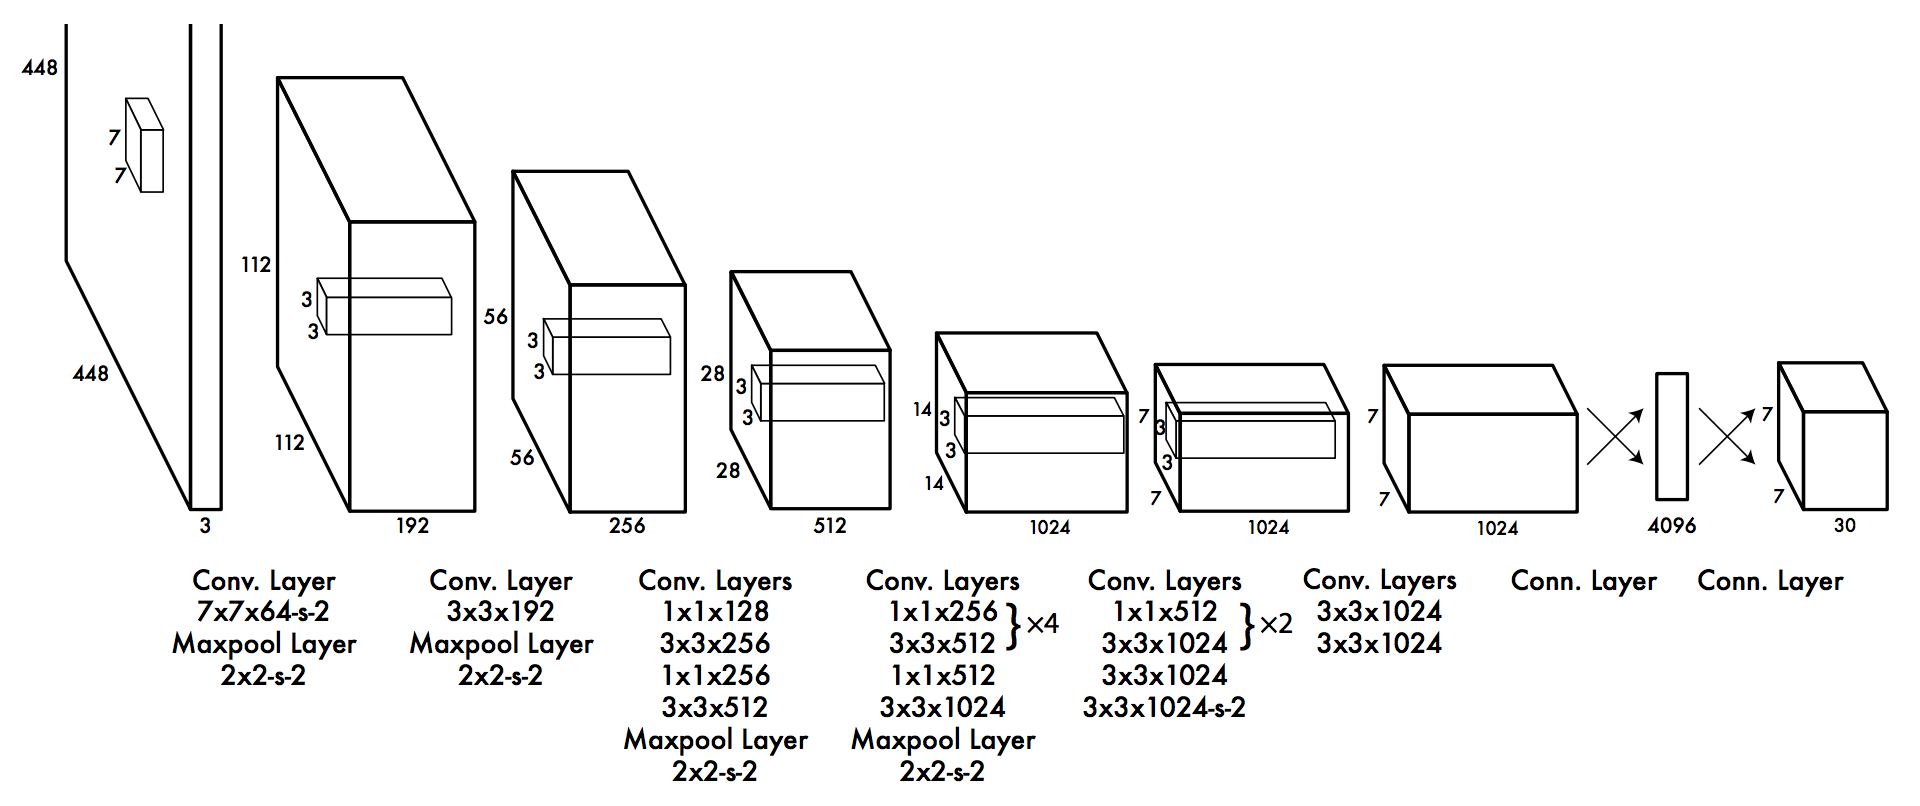
\includegraphics[width=0.8\textwidth]{images/yolo.png}
  \caption{Estructura de red del modelo YOLO \cite{art:yolo}.}
  \label{fig:yoloArch}
\end{figure}

\newpage